\documentclass[tikz, border = 1in]{standalone}

\usepackage{ geometry}

%\geometry{margin=1.0in}

\usepackage{tikz-uml}


\begin{document}
\pagenumbering{gobble}

%\pdfpagewidth 22in
%\pdfpageheight 16in

\begin{tikzpicture}



\umlclass[x = 0, y = 26]{network}{
+ networkName: str\\
+ nodes: list \\
+ paths: list 
}{
+ \_\_init\_\_(self, networkName): self\\
+ showNetworkName(self): networkName \\ 
+ addNodeList(self, nodeList): self \\
+ addPathList(self, pathList): self \\
+ nNodes(self): nNodes \\
+ selfPopulatePaths(self): self 
 }


\umlclass[x = 12, y = 22]{node}{
+ nodeName: str \\
+ pathsIn: list\\
+ pathsOut: list
}{
+ \_\_init\_\_(self, nodeName, timePeriod): self\\
+ addPathsOut(self, pathsOut): self.pathsOut \\
+ addPathsInt(self, pathsIn): self.pathsIn \\
+ showPathsOut(self): pathsOut\\
+ showPathsIn(self): pathsIn \\
+ showNodeName(self): nodeName}


\umlclass[x = 22, y = 22]{path}{
+ pathName: str \\
+ startNode: str\\
+ endEnd: str
}{
+ \_\_init\_\_(self, pathName): self\\
+ showEndNode(self): endNode\\
+ showStartNode(self): startNode \\
+ showPathName(self): pathName
 }

\umlunicompo[geometry=-|]{node}{network}
\umlunicompo[geometry=|-]{path}{network}


\umlclass[x = 22, y = 16]{populatedPath}{
+ groups: list
}{
+ \_\_init\_\_(self, pathName): self
 }

\umlimpl{populatedPath}{path}


\umlclass[x = 12, y = 13]{populatedNode}{
// Only only one group per Node  \\
+ groups: list \\
+ pathsOut: dict \\
+ nodeBiomass: float \\
}{
+ \_\_init\_\_(self, nodeName): self\\
+ addPathsOut(sefl): self.pathsOut \\
+ updateGroup(self): self \\ 
+ projectGroups(self):\\ 
+ calculateNodeBiomass( groups): self.biomass \\
+ calculateNodePop(self):  self \\
+ showNodePop(self): array \\
+ density(self): array \\
+ showNodeBiomass(self): array \\
}
 
 \umlimpl{populatedNode}{node}



\umlclass[x = 0, y = 18]{populatedNetwork}{
+ nYears: int \\
+ nPoints: int \\
+ minLength: float\\
+ maxLength: float\\
+ omega: np.array \\
+ hWidth: float \\
}{
+ \_\_init\_\_(self, networkName): self  \\
+ runSimulation(self): self \\
+ moveGroups(self): self \\
+ showNetworkPop(sefl): array \\
+ calculateNetworkPop(self): self \\
+ describeNetwork: print to screen\\
+ plotAllNodes: print to screen \\
+ setupNetworkMesh(nPoints, minLength, maxLength): self.omega \\
 }
 
 \umlimpl[anchor1 = 120, anchor2 = -120]{populatedNetwork}{network}

\umlunicompo[geometry=-|]{populatedNode}{populatedNetwork}
\umlunicompo[geometry=|-, anchor1 = 120]{populatedPath}{populatedNetwork}

\umlclass[x = 22, y = 6]{group}{
+ name: str\\
+ popDist: np.array \\ 
+ popDist0: np.array \\
+ survival: array or float\\
+ growth: array or float\\
+ probability: array or float\\
+ lengthWeight: array or float\\
+ density: array or float
}{
+ \_\_init\_\_(self, nodeName): self\\
+ showGroupName(name): name \\ 
+ createPopDist(nYears, nPoints, popDist): self\\
+ showPopDist(self): self.popDist\\
+ showPopDistYear(year): self.popDist[ year, :] \\
+ updatePopDistYear(year, popAdd): self \\
 }
 
  
 \umlunicompo{group}{populatedNode}
 
 \umlclass[x = 22, y = 12.5]{populatedHelpers}{
}{
+ addGroups(self, groups): self \\
+ showGroups(self): list \\
+ setLengthWeight(lengthWeight): self \\
+ createPopDist( nYears, nPoints, popDist0): self \\
+ showPop(self): array \\
+ showPopDist(self): array \\
+ updatePopDistYear( year, popAdd): self \\
 }

\umlimpl{populatedNode}{populatedHelpers}
\umlimpl{populatedPath}{populatedHelpers}
\umlimpl{group}{populatedHelpers}
 
 
   \umlclass[x = 30, y = 10]{lengthWeight}{
+ alphaLW: float\\
+ betaLW: float
}{
+ \_\_init\_\_(self, alphaLW, betaLW): self \\
+ \_\_call\_\_(self, omega): float
}

\umlunicompo{lengthWeight}{group}
\umlunicompo[geometry= -|, anchor2 = -70]{lengthWeight}{populatedNode}


 

 
 \umlclass[x = 30, y = 6.5]{densityNegExp}{
+ a: float \\ 
+ b: float
}{
+ \_\_init\_\_(self, a, b): self \\ 
+ \_\_call\_\_(self, biomass): float
}
 
\umlunicompo{densityNegExp}{group}
 
 
\umlclass[x = 30, y = 3]{logistic}{
+ alphaL: float \\ 
+ betaL: float\\ 
+ minL: float\\ 
+ maxL: float
}{
+\_\_init\_\_(self, aG, kG, sigmaG): self \\ 
+ \_\_call\_\_(z): float
}


\umlunicompo{logistic}{group}



\umlclass[x = 30, y = -1]{growthVB}{
+ aG: float \\
+ kG: float \\
+ sigmaG: float \\
}{
+ \_\_init\_\_(self, aG, kG, sigmaG): self \\
+ \_\_call\_\_(self, tzIn, zPrimeIn): float
}


\umlunicompo{growthVB}{group}

\umlclass[x = 30, y = -5]{linearRecruitment}{
+ lengthWeight: function\\
+ survival: function \\
+ probabilityReproducing: function \\
+ eggTransition: float \\
+ eggPerkg: float\\
+ muJ: float \\
+ sigmaJ: float \\ 
}{
+ \_\_init\_\_(self, omega, survival,  probabilityReproducing, eggTransition, eggPerk, muJ, sigmaJ ): self \\
+ \_\_call\_\_(self, omega, omegaPrime): float or array
}

\umlunicompo[anchor1 = 0, geometry = -|-]{linearRecruitment}{group}
 
 \umlclass[x = 22, y = 0]{groupWithSex}{
+ sex: str\\
+ contributeToReproduction: Bool \\
}{
+ \_\_init\_\_(self, nodeName): self \\
+ add(sex): self \\
+ show(sex): self.sex \\
+ addContributeToReproduction(self):  \\
+ showContributeToReproduction(self): 
 }
 
  \umlimpl{groupWithSex}{group}



\umlclass[x = 12, y = 6]{populatedNodeWithSex}{
// Multiple groups per node possible \\
+ sexClasses: list \\
+ femaleSexClasses: list 
}{
+ updateGroup(self, sexClasses, femaleSexClasses): self \\ 
 }
 
 \umlimpl{populatedNodeWithSex}{populatedNode}

\umlclass[x = 12, y =0]{populatedNodeWithSexSpecificParameter}{
+ impactedParametersBySex: dict \\ 
}{
+ updateGroup(self): self \\ 
 }
 
 \umlimpl{populatedNodeWithSexSpecificParameter}{populatedNodeWithSex}


\umlclass[x = 0, y = 08]{createNetworkFromCSVs}{
+ network: networkObject \\
}{
+ \_\_init\_\_(self, networkName): self  \\
+ pathOutListFunction( pathsOut, pathsOutProb): \{ pathsOut\} \\
+ showNetwork(self): networkObject\\
+ 
 }
\umlunicompo[anchor1 = 0, geometry = -|-]{linearRecruitment}{group}

%\umlclass[x = 12, y = 0]{group}{
%+ popLenDist: np.array \\
%+ groupProduceEggs: Bool\\
%+ groupImpactSexRatio: Bool\\
%+ groupImpactViability: Bool\\
%+ nYears: int\\
%+ groupSex: str\\
%+ groupName: str\\
%+ popSize:np.array\\
%+ popLenDist: np.array\\
%+ survival: np.array or float\\
%+ growth: np.array \\
%+ recruitment: np.array \\
%+ density: np.array\\
%+ lengthWeight: np.array\\
%+ groupOffspringPfemale: float\\
%+ groupOffspringViability = float\\
%+ omega: np.array\\
%+ hWidth: float\\
%+ pulseIntroductionString: np.array 
%}{
%+ \_\_init\_\_(self, groupName, popSize0, popLengDist0, omega, \\ nYears, survival, growth, \\recruitment, density, lengthweight): self \\
%+ timeStepGroup(self, t, tPlusOne, pReferenceGroupBirth, \\offspringViability, recruitGroup,\\ popLenDistbiomass, referenceSex): self \\
%+ movement(self, immigration, emigration, t): self \\ 
%+ showGroupPopSize(self): popSize\\
%+ showGroupProduceEggs(self): groupProduceEggs\\
%+ showGroupName(self): groupName\\
%+ showGroupSex(self): groupSex\\
%+ plotLengthTime(self): plots\\
%+ plotPop(self): plot
%}
%


%\umlclass[x = 38, y = 5]{logistic}{
%+ alphaL: float \\ 
%+ betaL: float\\ 
%+ minL: float\\ 
%+ maxL: float
%}{
%+\_\_init\_\_(self, aG, kG, sigmaG): self \\ 
%+ \_\_call\_\_(z): float
%}
%
%
%\umlclass[x = 30, y = 6]{survival}{
%+ alphaS: float \\ 
%+ betaS: float\\ 
%+ minS: float\\ 
%+ maxS: float
%}{
%+ \_\_call\_\_(self, z): float
%}
%
%\umlclass[x = 40, y = 12]{probabilityOfReproducing}{
%+ alphaL: float \\ 
%+ betaL: float\\ 
%+ minL: float\\ 
%+ maxL: float
%}{
%+ \_\_call\_\_(self, z): float
%}
%
%\umlclass[x = 32, y = 12]{linearRecruitment}{
%+ juvenile: np.array \\
%+ lenghtWeight: np.array\\
%+ survival: float or np.array \\
%+ probabilityReproducing: float or np.array\\
%+ eggTransition: float\\
%+ eggPerkg: float 
%}{
%+ \_\_init\_\_(self, omega, lengthWeight, \\ probabilityReproducing, \\ eggTransition, eggPerkg, muJ, sigmaJ): self \\
%+ \_\_self\_\_(self, omega, omegaPrime): np.array \\
%}
%
%\umlclass[x = 24, y = 10]{lengthWeight}{
%+ alphaLW: float\\
%+ betaLW: float
%}{
%+ \_\_init\_\_(self, alphaLW, betaLW): self \\
%+ \_\_call\_\_(self, omega): float
%}
%
%
%\umlclass[x = 0, y = 1]{growthVB}{
%+ aG: float \\
%+ kG: float \\
%+ sigmaG: float \\
%}{
%+ \_\_init\_\_(self, aG, kG, sigmaG): self \\
%+ \_\_call\_\_(self, tzIn, zPrimeIn): float
%}
%
%
%\umlclass[x = 30, y = 22]{helpers}{
%}{
%+ pathOutListFunction( pathsOut, pathsOutProb): dict\\
%+ initializeModelFromCSVs(dfNetwork, dfNode, dfGroups): networkModel 
%}
%
%
%\umlclass[x = 0, y = 6]{densityNegExp}{
%+ a: float \\ 
%+ b: float
%}{
%+ \_\_init\_\_(self, a, b): self \\ 
%+ \_\_call\_\_(self, biomass): float
%}
%
%
%\umlclass[x = 0, y = 10]{densityNone}{
%}{
%+ \_\_call\_\_(self, biomass): 1
%}
%
%
%
%\
%\umlimpl{probabilityOfReproducing}{logistic}
%
%
%\umlunicompo{survival}{linearRecruitment}
%\umlunicompo{probabilityOfReproducing}{linearRecruitment}
%\umlunicompo{lengthWeight}{linearRecruitment}
%
%
%
%\umlunicompo{survival}{group}
%\umlunicompo{lengthWeight}{group}
%\umlunicompo{linearRecruitment}{group}
%
%
%\umlunicompo{growthVB}{group}
%\umlunicompo{densityNegExp}{group}
%
%
%\umlimpl{densityNone}{densityNegExp}
%
%\umlreal[stereo = builds]{helpers}{networkModel}

\end{tikzpicture}

\end{document}